\documentclass{beamer}
\usetheme{Boadilla}
%\usetheme{Warsaw}
%\setbeamercovered{transparent}
\beamertemplatetransparentcoveredhigh
\usepackage[portuges]{babel}
\usepackage[utf8]{inputenc}
\usepackage[alf]{abntex2cite}	
\usepackage{lmodern}
\usepackage[T1]{fontenc}
\usepackage[portuguese, linesnumbered, vlined, titlenumbered, ruled]{algorithm2e}
\SetKwRepeat{Registro}{registro \{}{\}}%
\usepackage{hyperref} 

% Macro que faz com que a numeracao de diferentes algoritmos continue de onde parou
\newcommand{\rememberlines}{\xdef\rememberedlines{\number\value{AlgoLine}}}
\newcommand{\resumenumbering}{\setcounter{AlgoLine}{\rememberedlines}}


\title[Aula Prática Algoritmos de Ordenação]{Estrutura de Dados}
\subtitle{Grafos}
\author[Frederico Santos de Oliveira]{prof. Frederico Santos de Oliveira}
\institute[UFMT]{Universidade Federal de Mato Grosso\\ Instituto de Engenharia}
\date{}


\begin{document}

\begin{frame}
\titlepage % Print the title page as the first slide

\begin{figure}[!h]
  \centering
   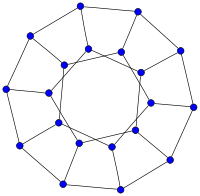
\includegraphics[width=80pt]{imagens/introducao.png}
  \label{fig_introducao}
\end{figure}
\end{frame}

%\section*{Roteiro}

\begin{frame}
  \frametitle{Agenda}
  \tableofcontents
\end{frame}

%------------------------------------------------
\section{Introdução}
%------------------------------------------------

\section{Representação}

\begin{frame}{Representação}
As principais formas para representar grafos são:
\begin{itemize}
\item {\bf Matriz de Adjacência}
\item {\bf Lista de Adjacência}
\end{itemize}
\end{frame}


\subsection{Matriz de Adjacência}

\begin{frame}{Representação}{Matriz de Adjacência}
\begin{itemize}
\item A {\bf Matriz de Adjacência} de um grafo $G = (V, A)$ contendo n vértices é uma matriz $n \times n$ de bits, onde $A[i, j]$ é $1$ (ou verdadeiro) se e somente se existe um arco do vértice $i$ para o vértice $j$.
\item Para grafos ponderados $A[i, j]$ contém o rótulo ou peso associado com a aresta e, neste caso, a matriz não é de bits.
\item Se não existir uma aresta de $i$ para $j$ então é necessário utilizar um valor que não possa ser usado como rótulo ou peso.
\end{itemize}
\end{frame}

\begin{frame}{Representação}{Matriz de Adjacência}
\begin{figure}[!h]
  \centering
  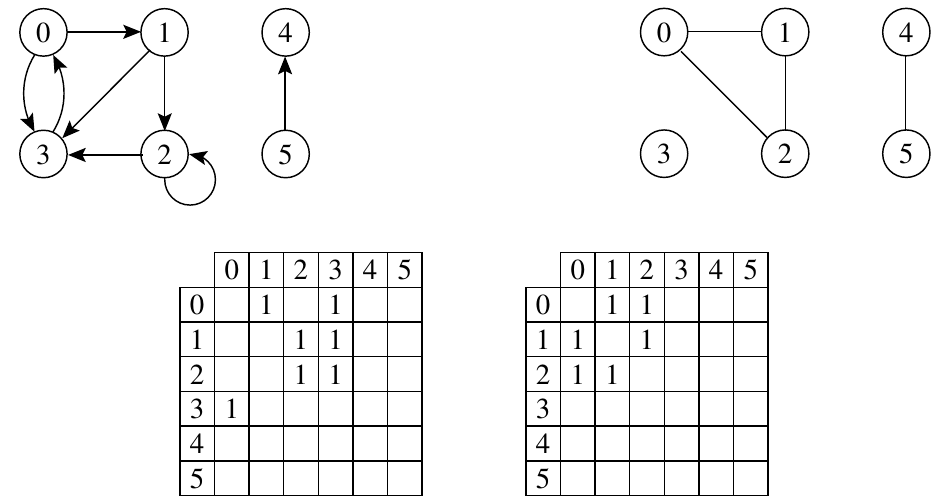
\includegraphics[width=300pt]{imagens/exemplo_matriz_adjacencia.png}
  \label{fig_exemplo_matriz_adjacencia}
\end{figure}
\end{frame}


\subsection{Lista de Adjacência}

\begin{frame}{Representação}{Lista de Adjacência}
\begin{itemize}
\item A {\bf Lista de Adjacência} consiste de um vetor, denominado $Adj$, contendo $|V|$ listas, uma para cada vértice de $V$.
\item Para cada $u \in V$, Adj[u] contém todos os vértices de $G$ adjacentes a $u$.
\item Os vértices são armazenados de forma arbitrária na lista.
\item Também pode ser utilizada para representar grafos dirigidos.
\end{itemize}
\end{frame}


\begin{frame}{Representação}{Lista de Adjacência}
\begin{figure}[!h]
  \centering
  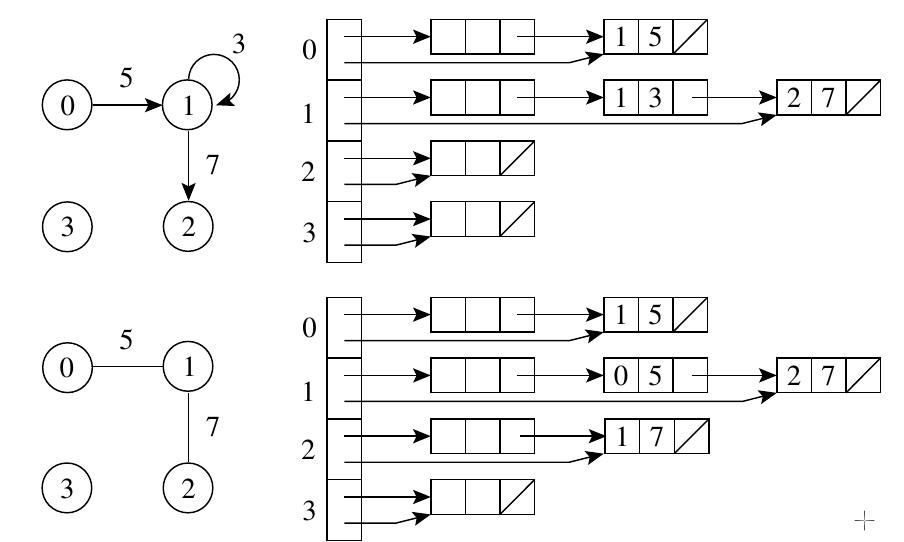
\includegraphics[width=300pt]{imagens/exemplo_lista_adjacencia.png}
  \label{fig_exemplo_lista_adjacencia}
\end{figure}
\end{frame}

%----------------------------------------------------------------------------------------
\section{Percurso}
%----------------------------------------------------------------------------------------

\begin{frame}{Percurso}
\begin{itemize}
\item Fazer buscas em um grafo significa percorrer suas arestas sistematicamente, de modo a visitar seus vértices.
\item As principais formas para percorrer grafos são:
\begin{itemize}
\item {\bf Busca em Largura} - em inglês {\it Breadth-First Search} ou BFS
\item {\bf Busca em Profundidade} - em inglês {\it Depth-First Search} ou DFS
\end{itemize}
\end{itemize}
\end{frame}

%----------------------------------------------------------------------------------------
\subsection{Busca em Largura}
%----------------------------------------------------------------------------------------

\begin{frame}{Percurso}{Busca em Largura}
\begin{itemize}
\item A {\bf Busca em Largura} é um dos algoritmos mais simples para exploração de um grafo.
\begin{itemize}
\item Dados um grafo G = (V, E) e um vértice $s$, chamado de fonte, a busca em largura sistematicamente explora as arestas de $G$ de maneira a visitar todos os vértices alcançáveis a partir de $s$.
\end{itemize}
\item  Expande a fronteira entre vértices descobertos e não-descobertos uniformemente através da largura da fronteira.
  \begin{itemize}
  \item O algoritmo descobre todos os vértices a uma distância $k$ do vértice de origem $s$ antes de descobrir qualquer vértice a uma distância $k + 1$.
  \end{itemize}
\item O grafo pode ser direcionado ou não-direcionado.
\item Esse algoritmo é base para o algoritmo de Dijkstra, o qual encontra o menor caminho de um vértice aos demais.
\end{itemize}
\end{frame}


\begin{frame}{Percurso}{Busca em Largura}
\scalebox{0.6}{
\begin{algorithm}[H]
\caption{BuscaEmLargura} 
\label{BuscaEmLargura}
\Entrada{Grafo $G = (V,A)$, vértice inicial $s$.}
\Saida{Percurso armazenado no campo ``predecessor'' presente em cada vértice $v \in V$.}
\Inicio{
  \Para {cada vértice $u \in V$} {
    $u.cor \leftarrow$ Branco \\
    $u.d \leftarrow \infty$ \\ 
    $u.\pi \leftarrow$ NULL \\
  }
  $s.cor \leftarrow$ Cinza \\
  $s.d \leftarrow$ 0 \\
  $s.\pi \leftarrow$ NULL \\
  CriaFilaVazia(Q) \\
  Enfileira(Q, s) \\
  \Enqto{($Q \neq \emptyset$)} {
    u $\leftarrow$ Desenfileira(Q) \\
    \Para {cada vértice $v \in u.ListaAdj$} {
      \Se{v.cor = Branco} {
			v.cor $\leftarrow$ Cinza \\
			v.d $\leftarrow$ u.d + 1 \\
			$v.\pi \leftarrow$ u \\
			Enfileira(Q, v)\\
      }
    }
    u.cor $\leftarrow$ Preto \\
  }
}
\end{algorithm}
}  

\tiny{Adaptado de \citeonline{Cormen2012}.}
\end{frame}

%----------------------------------------------------------------------------------------
\subsection{Busca em Profundidade}
%----------------------------------------------------------------------------------------

\begin{frame}{Percurso}{Busca em Profundidade}
\begin{itemize}
\item Na {\bf Busca em Profundidade}, a estratégia é buscar o vértice mais profundo no grafo sempre que possível:
\begin{itemize}
\item As arestas são exploradas a partir do vértice $v$ mais recentemente descoberto que ainda possui arestas não exploradas saindo dele.
\end{itemize}
\item Quando todas as arestas adjacentes a v tiverem sido exploradas a busca anda para trás para explorar vértices que
saem do vértice do qual $v$ foi descoberto ({\it backtracking}).
\item O algoritmo é a base para muitos outros algoritmos importantes, tais como:
\begin{itemize}
\item Verificação de grafos acíclicos, 
\item Ordenação topológica e 
\item Componentes fortemente conectados.
\end{itemize} 
\end{itemize}
\end{frame}

%----------------------------------------------------------------------------------------

\begin{frame}{Percurso}{Busca em Profundidade}
\begin{columns}
\begin{column}{0.5\textwidth}
  \scalebox{0.8}{
  \begin{algorithm}[H]
  \caption{BuscaEmProfundidade} 
  \label{BuscaEmprofundidade}
  \Entrada{Grafo $G = (V,A)$.}
  \Saida{Percurso armazenado no campo ``predecessor'' presente em cada vértice $v \in V$.}
  \Inicio{
    \Para {cada vértice $u \in V$} {
      $u.cor \leftarrow$ Branco \\
      $u.\pi \leftarrow$ NULL \\
    }
    tempo $\leftarrow$ 0\\
    \Para {cada vértice $u \in V$} { 
      \Se {u.cor = Branco} {
		DFS-Visita(u)\\
      }
    }
  }
  \end{algorithm}
  }
\end{column}
\begin{column}{0.5\textwidth}  
    \begin{center}
  \scalebox{0.8}{
  \begin{algorithm}[H]
  \caption{DFS-Visita} 
  \label{Visita}
  \Entrada{Grafo $G = (V,A)$, vértice inicial $s$.}
  % \Saida{Percurso armazenado no campo ``predecessor'' presente em cada vértice $v \in V$.}
  \Inicio{
    tempo $\leftarrow$ tempo + 1\\
    $u.d \leftarrow$ tempo \\      
    $u.cor \leftarrow$ Cinza \\
    \Para {cada vértice $v \in u.ListaAdj$} { 
      \Se {v.cor = Branco} {
		$v.\pi \leftarrow u$ \\
		DFS-Visita(G, v)\\
      }
    }
    u.cor $\leftarrow$ Preto \\
    tempo $\leftarrow$ tempo + 1\\
    u.f $\leftarrow$ tempo \\
  }
  \end{algorithm}
  }  
     \end{center}
\end{column}
\end{columns}
\tiny{Adaptado de \citeonline{Cormen2012}.}
\end{frame}

%----------------------------------------------------------------------------------------

\begin{frame}
\Huge{\centerline{Dúvidas?}}

\begin{figure}[!h]
  \centering
  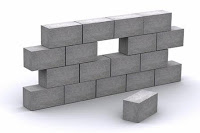
\includegraphics[width=100pt]{imagens/duvidas.jpg}
  \label{fig_fim}
\end{figure}
\end{frame}

%------------------------------------------------

\section{Referências bibliográficas}
  \frame{\frametitle{Referências bibliográficas}
    \bibliographystyle{abntex2-alf}
    \bibliography{referencias}
  }

%------------------------------------------------
\section{Material Complementar}
%------------------------------------------------

\begin{frame}{Material Complementar}
   \begin{itemize}
	\item Material IME
	\begin{itemize}
   \item \href{https://www.ime.usp.br/~pf/algoritmos_para_grafos/aulas/bfs.html}{https://www.ime.usp.br/~pf/algoritmos\_para\_grafos/aulas/bfs.html}      
   \item \href{https://www.ime.usp.br/~pf/algoritmos_para_grafos/aulas/dfs.html}{https://www.ime.usp.br/~pf/algoritmos\_para\_grafos/aulas/dfs.html}   	
	\end{itemize}		
   \item Animação Breadth-First Search (Busca em Largura)
   \begin{itemize}
   \item \href{https://www.cs.usfca.edu/~galles/visualization/BFS.html}{https://www.cs.usfca.edu/~galles/visualization/BFS.html}   
   \end{itemize}
   \item Animação Depth-First Search (Busca em Profundidade)
   \begin{itemize}
   \item \href{https://www.cs.usfca.edu/~galles/visualization/DFS.html}{https://www.cs.usfca.edu/~galles/visualization/DFS.html}   
   \end{itemize}
   \end{itemize}
\end{frame}    


\begin{frame}{Material Complementar}
   \begin{itemize}
	\item Youtube
	\begin{itemize}
   \item \href{https://www.youtube.com/watch?v=jWoP1fTTDzE}{Estrutura de Dados Descomplicada - Busca em Largura}      
   \item \href{https://www.youtube.com/watch?v=pJ3ilnhXWCQ}{Estrutura de Dados Descomplicada - Busca em Profundidade}   	
   \item \href{https://www.youtube.com/watch?v=MC0u4f334mI}{Univesp - Grafos}   
   \item \href{https://www.youtube.com/watch?v=9J3Sz6K--8c}{Univesp - Busca em Largura}      
   \item \href{https://www.youtube.com/watch?v=doH9o1sO-Cw}{Univesp - Busca em Profundidade}         
	\end{itemize}		
   \end{itemize}
\end{frame}    
%----------------------------------------------------------------------------------------
\end{document} 
